\chapter{Development}\label{development}

In the following chapter, the development process that followed the design phase and brought to the creation of the prototype of the whole system is described.

Some technological constraints were imposed from the requirements and the design phase.
In particular, the need for a lightweight Web application that didn't have to be installed on the user's machine and, from the MAS infrastructure point of view, the need to adhere to the JaCaMo platform, therefore to produce XML \moise{} specifications.

The development process was divided into three main parts.
First, the Web IDE was implemented to get continuous and fast feedback about the visual language.
Second, the backend and the specifications storage were developed to provide persistence to the organizations created by users.
Finally, the Web IDE was integrated with the runtime environment to allow the user to access information about the running agents and deploy the organizations.

The important details and choices about the implementation of the main component of the systems are described in the following sections.

\section{Web-based IDE}
Given that the main goal of the project is to provide non-technical users with an easy and intuitive tool to create and run organizations, the Web IDE is probably the most important component of the system together with the visual language.
Therefore, when users are confronted with the UI of the IDE they should be able to clearly understand what each component of the interface means and how to use it without any detailed explanation.

\begin{figure}
    \centering
    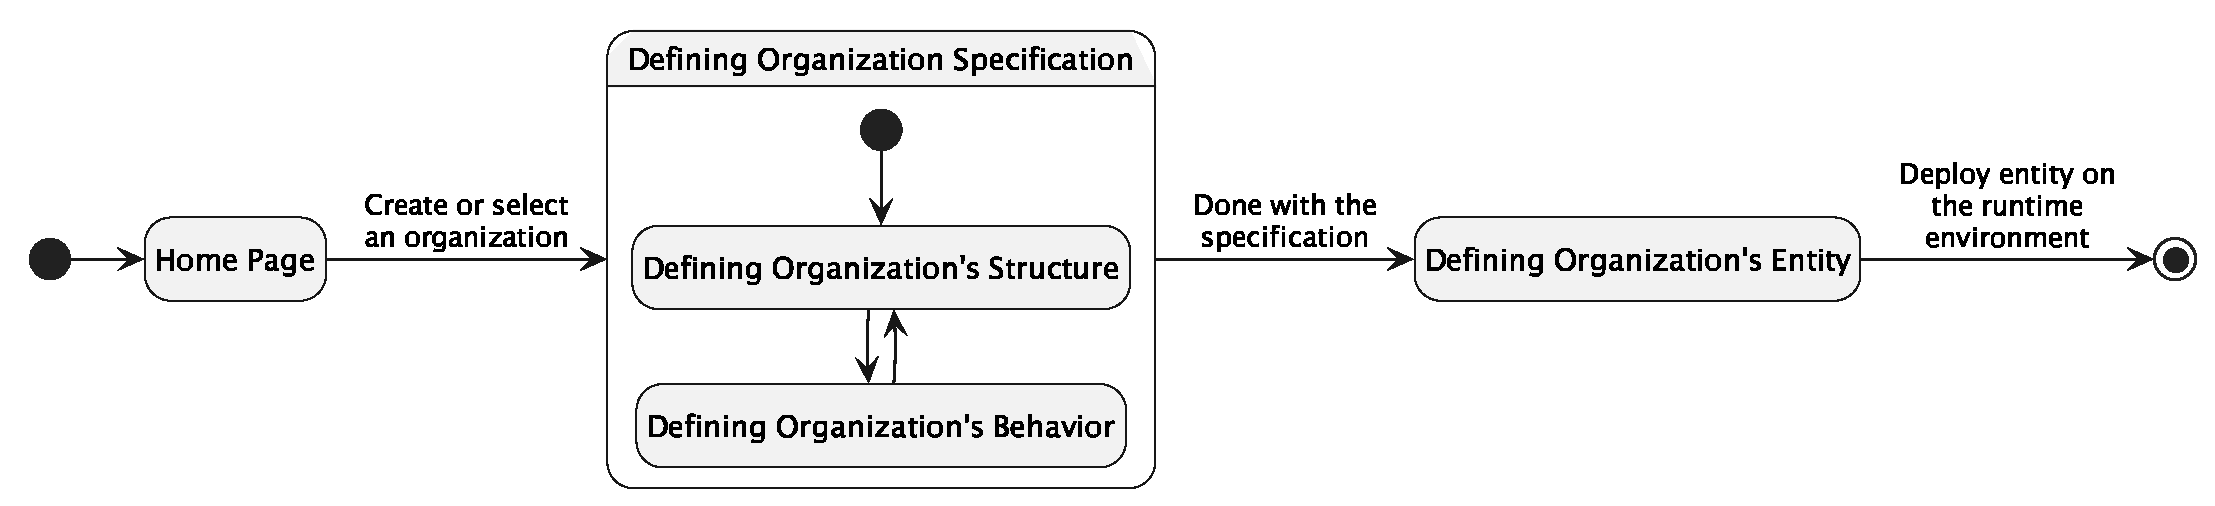
\includegraphics[width=\linewidth]{images/web-ide.eps}
    \caption{Typical workflow of a user utilizing the Web-based IDE.}
    \label{fig:ide}
\end{figure}

\subsection{Web User Interface}
As a starting point for the design of the UI, the typical workflow of a user that wants to create an organization is considered.

As shown in \cref{fig:ide}, the user starts by either creating a new organization or selecting an existing one.

Then, the user can define or edit the organization specification by using the designed visual language.
In particular, the user specifies the structure and the expected behavior of the organization in an iterative way.
Indeed, it is important to avoid sequentiality in the process as the user should feel free to easily navigate through the two separate diagrams and continuously modify them as the organization evolves.

Once the specification is ready, the user can define the organization entity by assigning the roles to the running agents. Finally, the organization can be deployed on the runtime environment and enforced on the agents.

Therefore, the final UI of the Web IDE consists of four main pages:
\begin{itemize}
    \item \textbf{Home Page} where the user can specify the name of the organization and create it or select an existing one.
    \item \textbf{Structural Diagram} where the user can define the structure of the organization.
    \item \textbf{Functional Diagram} where the user can define the expected behavior of the organization.
    \item \textbf{Entity Definition} where the user can assign the roles to the running agents and deploy the organization.
\end{itemize}

In \cref{fig:ide-structural-all} the UI of the Structural Diagram is shown.
As can be seen, the left panel contains the available elements that can be used to create the organization structure.
Indeed, the user can create new roles choosing whether they are concrete or abstract, and new groups.
Once a component has been created, it can be moved around the diagram and modified by clicking on it.
The click on a component opens a side menu that allows the user to edit the properties of the selected component.
In particular, \cref{fig:ide-structural-side} shows the side menu for the role \texttt{r1}.
Here the user can specify which role, if any, the selected role extends from, which group it belongs to, and the cardinality of the role in the group, i.e. the minimum and maximum number of agents that can be assigned to the role.

\begin{figure}
    \centering
    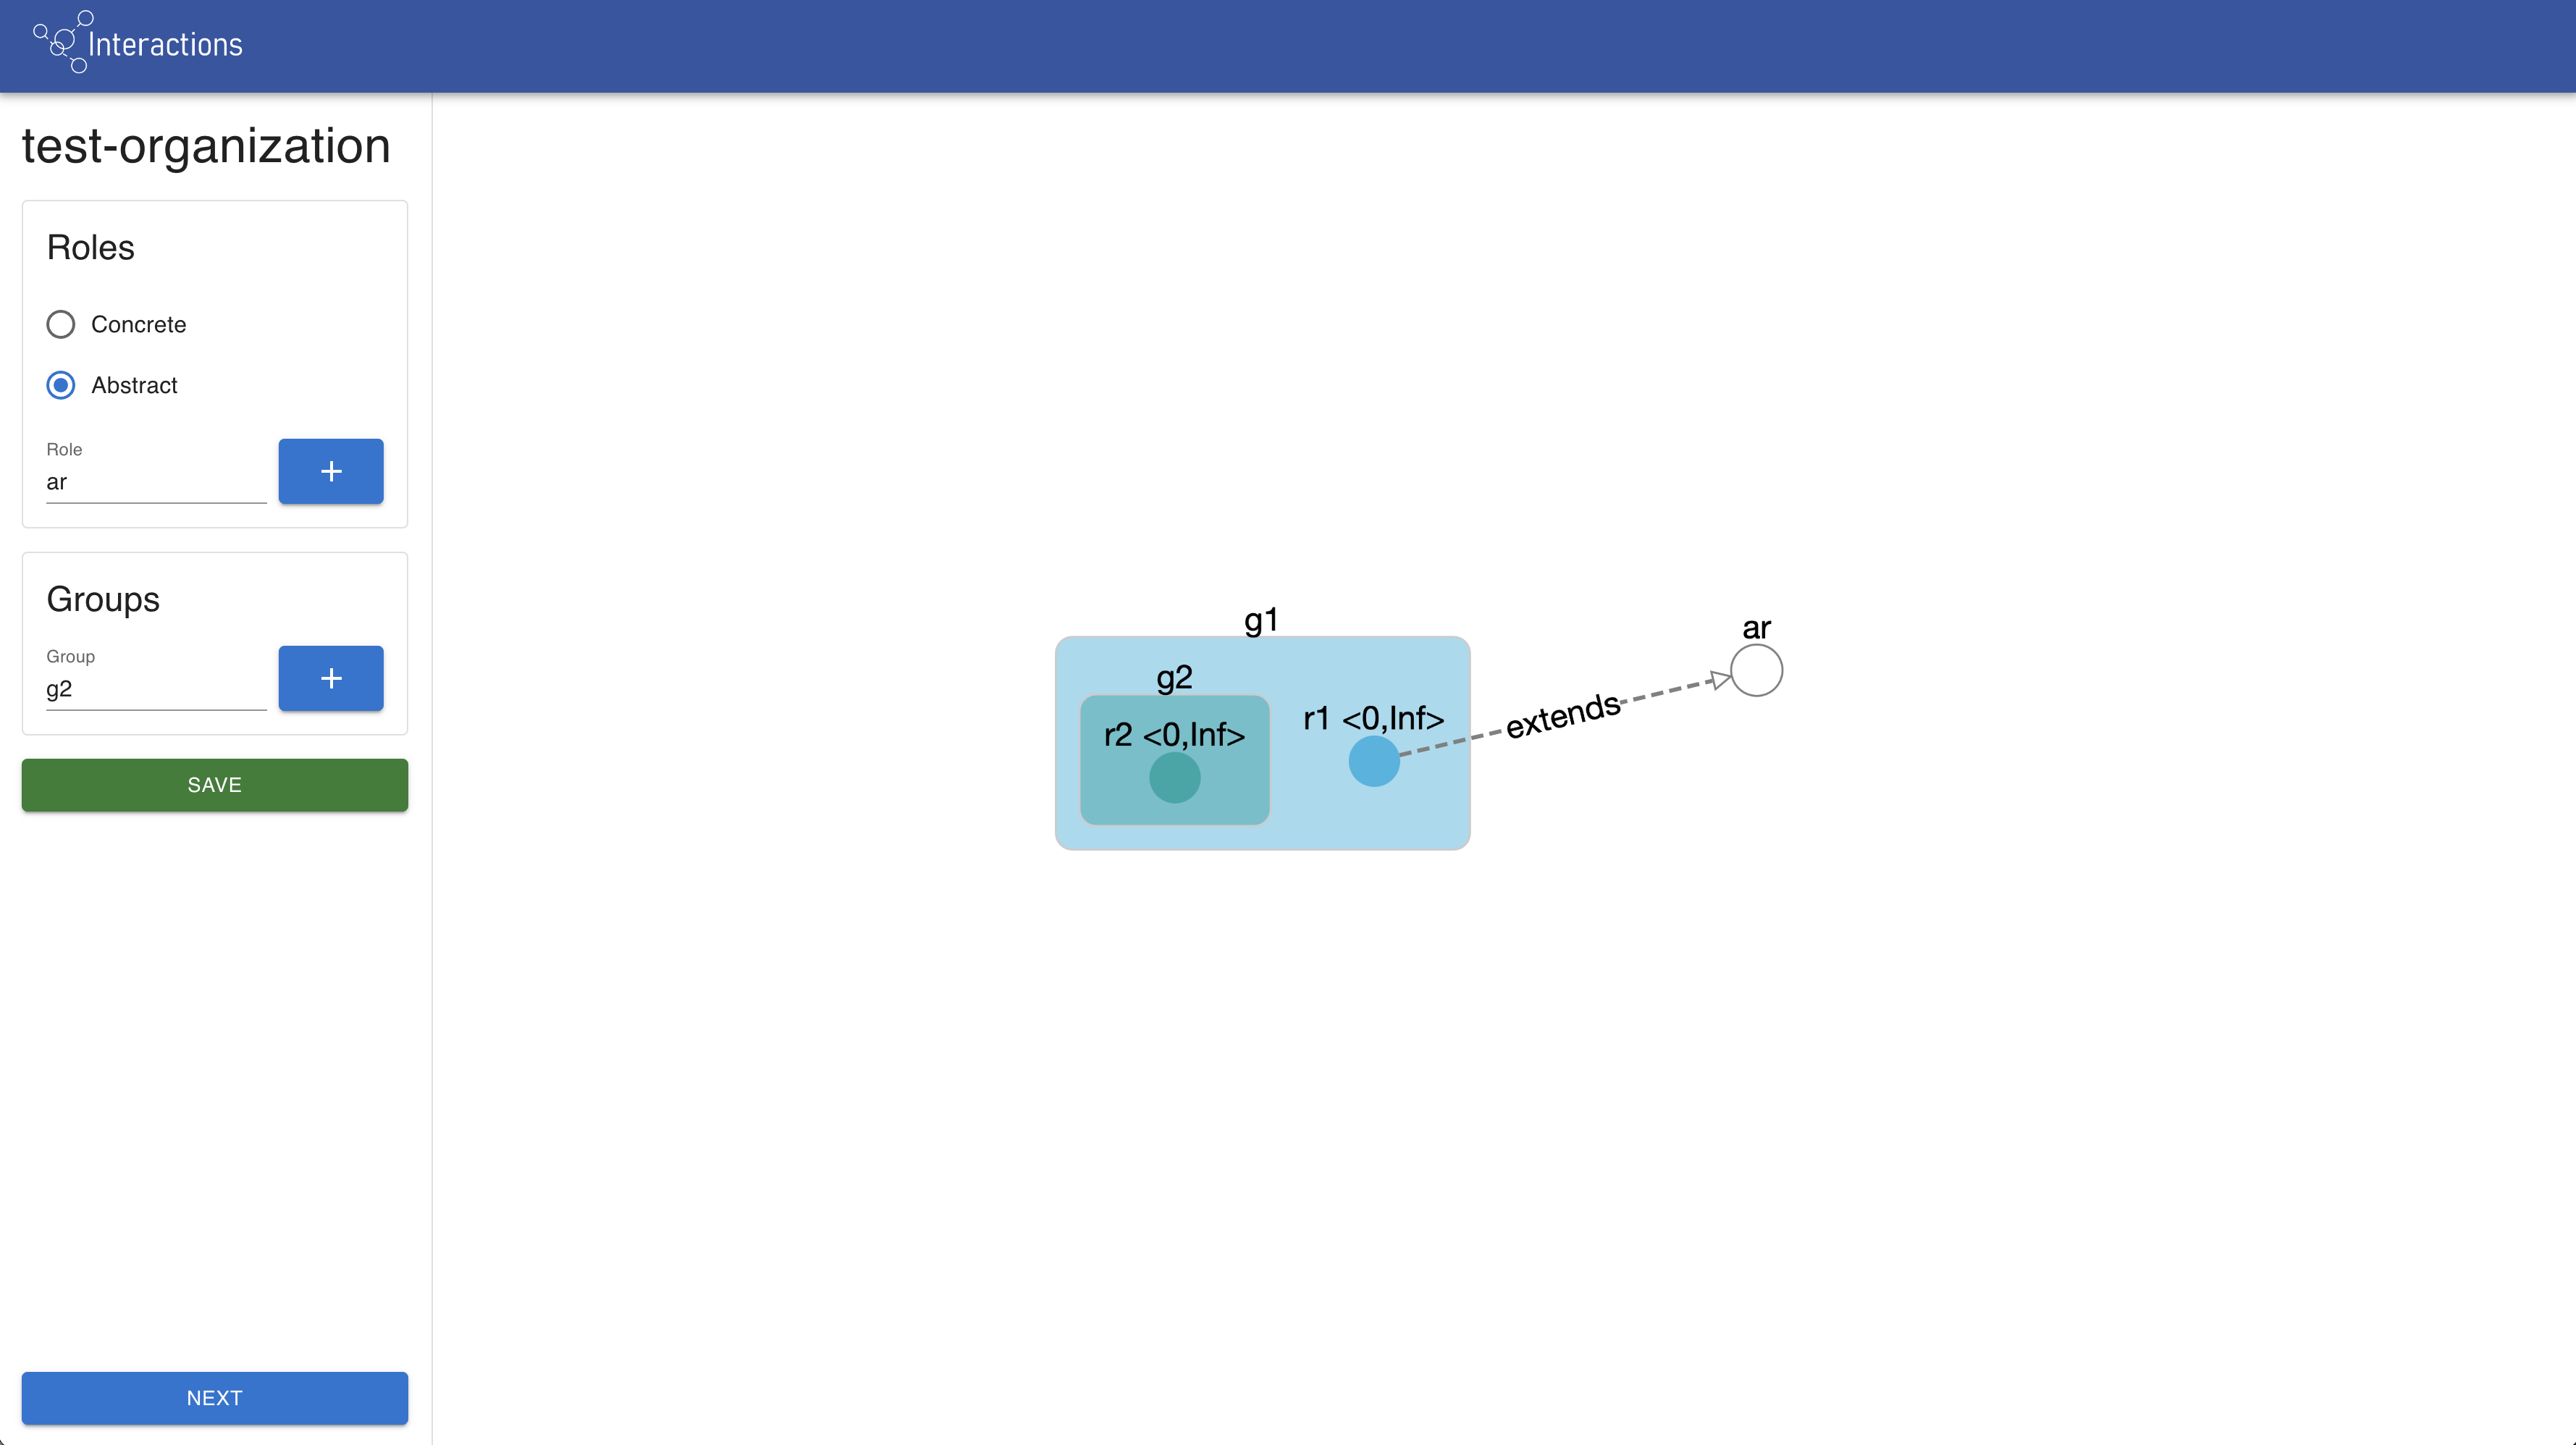
\includegraphics[width=\linewidth]{images/ide/structural.png}
    \caption{Structural Diagram of the Web IDE.}
    \label{fig:ide-structural-all}
\end{figure}

\begin{figure}
    \centering
    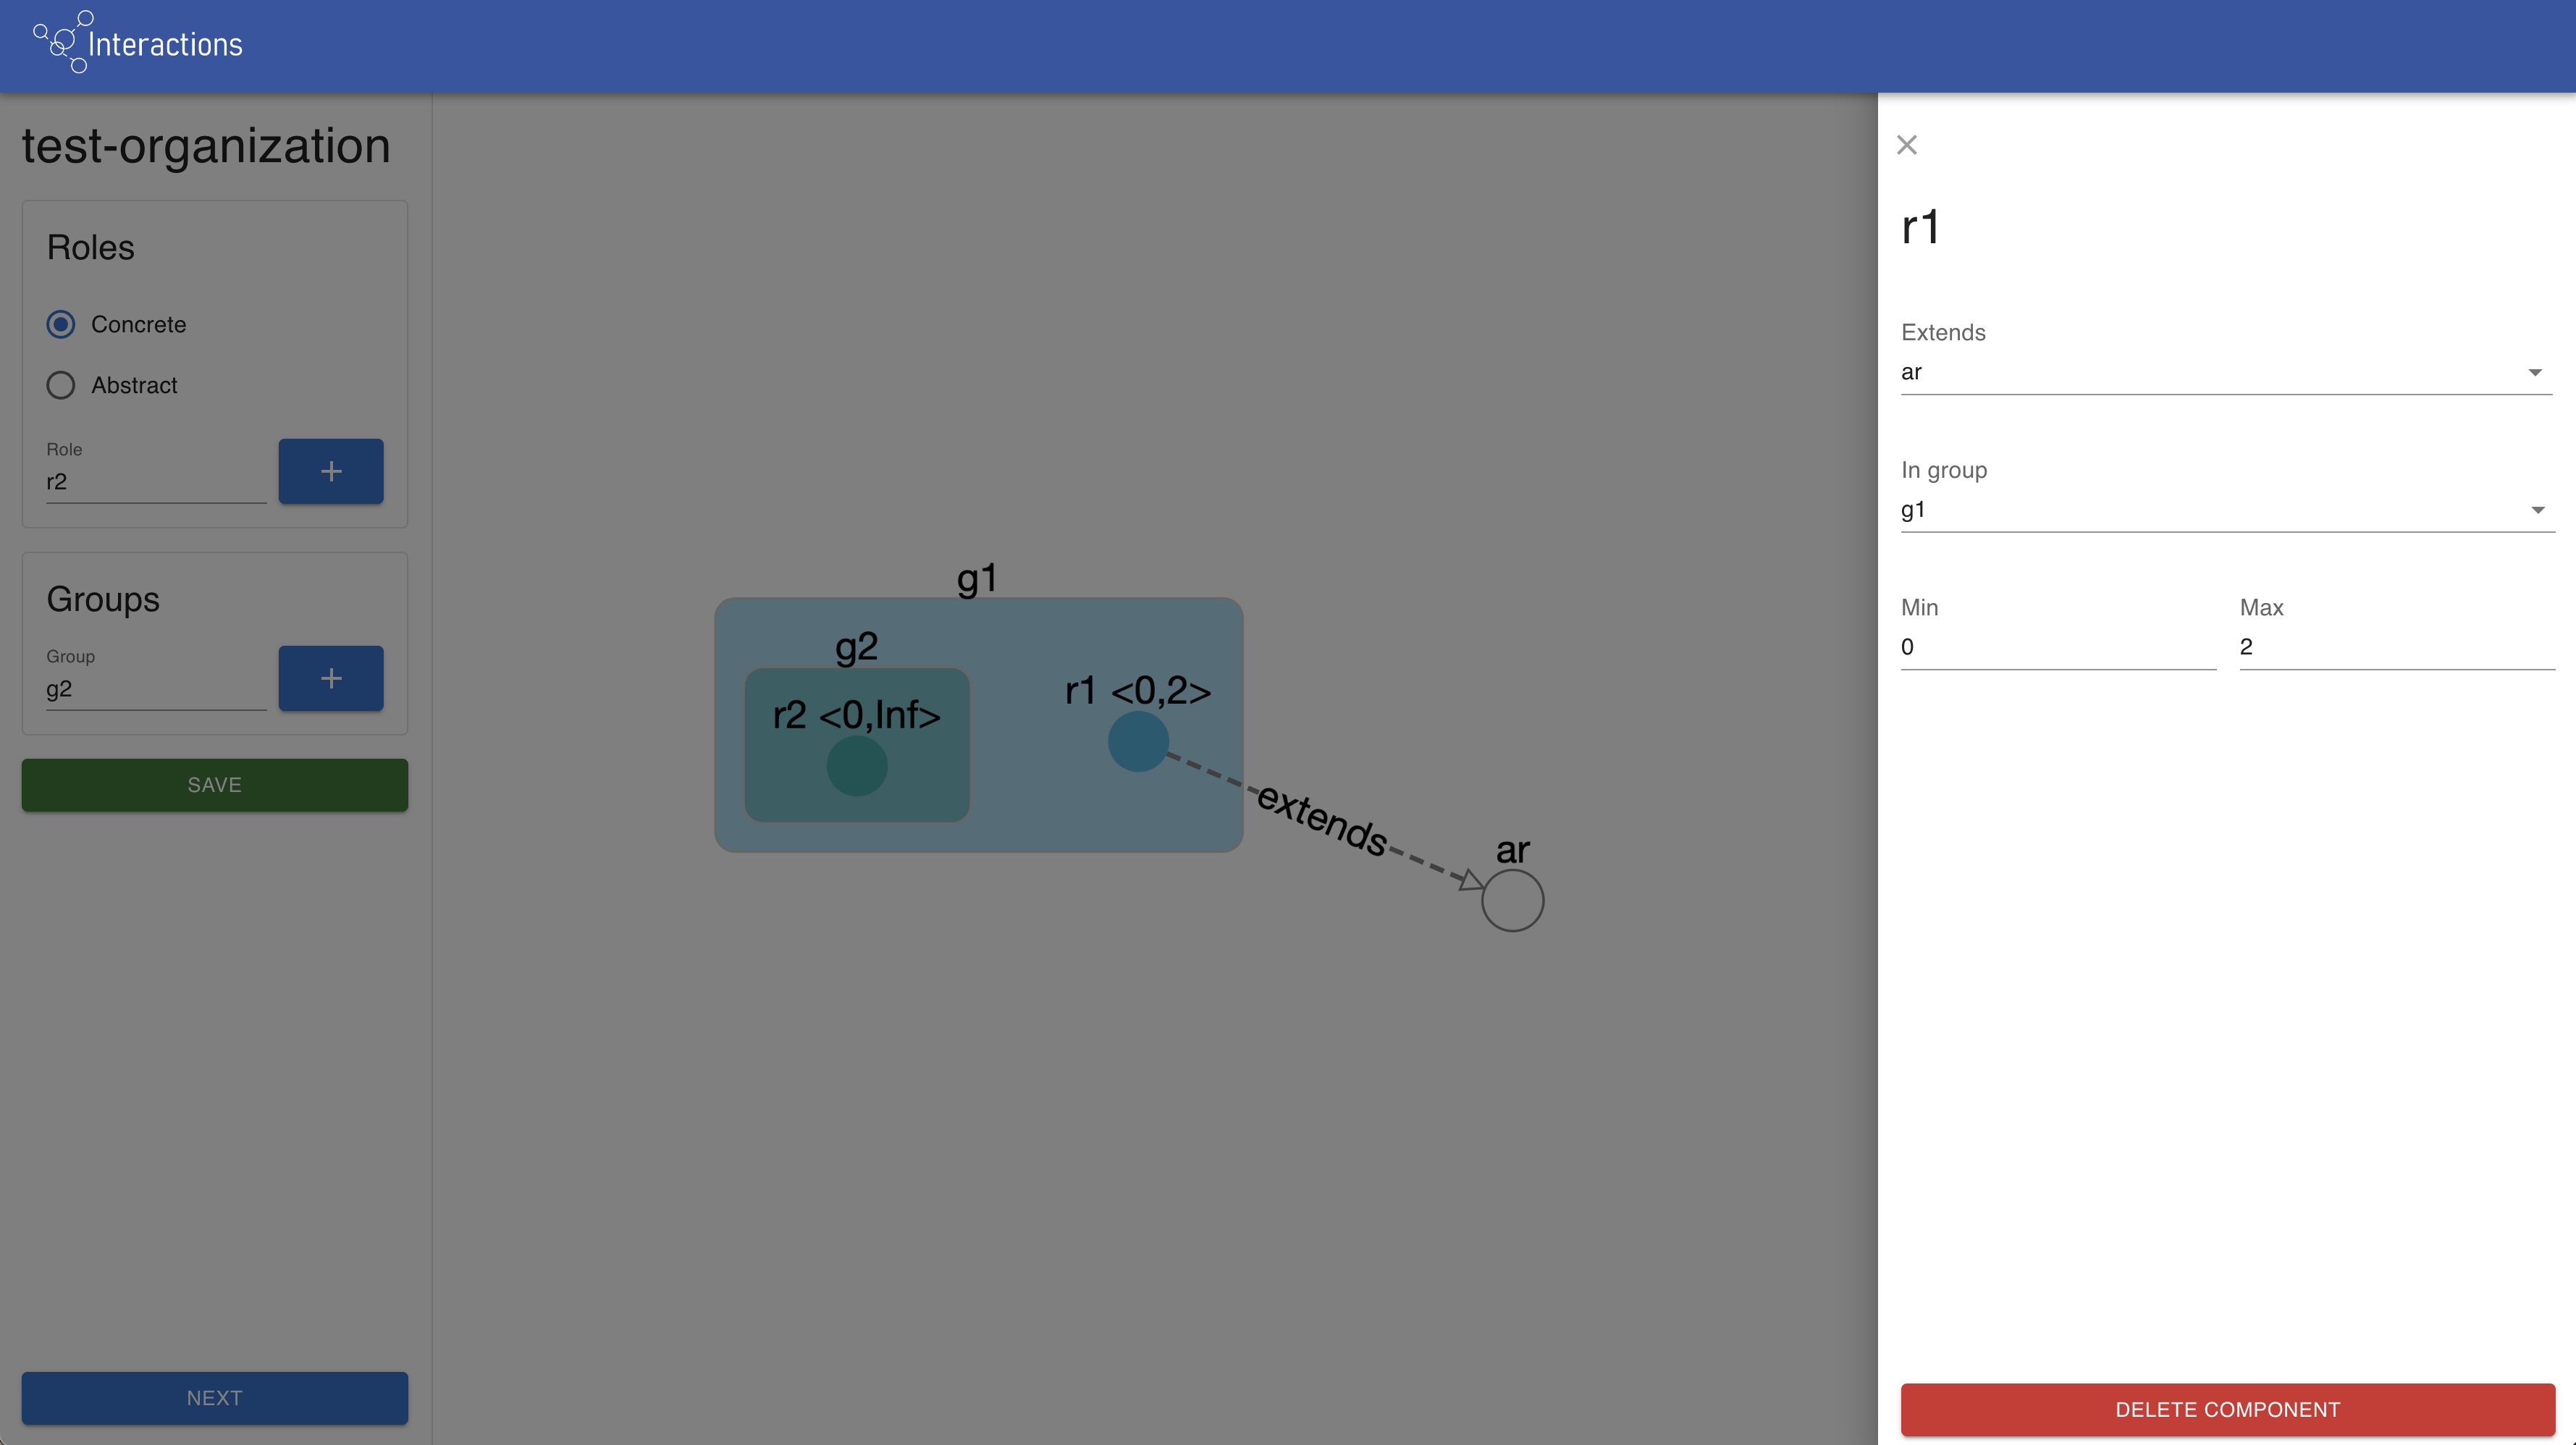
\includegraphics[width=\linewidth]{images/ide/structural-side.png}
    \caption{Detail showing the side menu in the Structural Diagram of the Web IDE.}
    \label{fig:ide-structural-side}
\end{figure}

\subsection{Technologies}
The following section describes the main technologies used to implement the Web IDE.

Since the component is based on Web technologies, the main two languages available for the implementation of the client-side logic are \textit{JavaScript}~\footnote{\url{https://developer.mozilla.org/en-US/docs/Web/javascript}} and \textit{TypeScript}~\footnote{\url{https://www.typescriptlang.org/}}.
The latter was created to address problems coming with developing large-scale applications, introducing static typing and object-oriented features.
Typescript's type-checking makes it easier to find and fix bugs, therefore, it was chosen as the language for the implementation of the Web IDE.

Moreover, a client-side framework was used to implement the Web-based IDE.
The main reason for this choice is that frameworks provide a set of tools that simplify the development of interactive Web applications.
They allow the developer to create reusable components that encapsulate the logic and the UI of a specific part of the application, therefore helping to divide the latter into smaller and more manageable parts and keeping the code clean and organized.
The one chosen for this project is \textit{React}~\footnote{\url{https://reactjs.org/}}.
Although there is no strong motivation for why it was preferred over others, React is probably the most popular, therefore, possible new contributors to the project will be more likely to be familiar with it.

To further facilitate the development of the UI, the \textit{Material-UI}~\footnote{\url{https://mui.com/}} library was used.
It implements Google's \textit{Material Design} and it provides a set of tested prebuilt components that are ready to be used in the application.

Finally, to make the implementation of the diagrams easier, the \textit{Cytoscape}~\footnote{\url{https://js.cytoscape.org/}} library was used.
It is a modular graph library that provides a set of tools to create and manipulate graphs and diagrams.
Using the library, together with a few extensions, made it possible to provide a simple and intuitive way to create and edit the diagrams.

\subsection{Code Generation}\label{sec:code-generation}
Since the specifications created by the user with the Web IDE have to be compatible with the JaCaMo platform, and in particular, with \moise{}, the diagrams have to be translated into XML files.
Equally important, actual \moise{} XML specification files have to be correctly parsed and translated into the corresponding visual representations.

Once the design phase of the different components of the visual language was in an advanced stage, the actual implementation of the code generation started.

The decision was to first implement the components that are present in both the Structural and Functional Diagrams.
This allowed for having a core domain that is unlikely to change in the future and that could be used as a starting point for both the translation into the visual components and XML tags.
In particular, the core domain consists of the components shown in \cref{fig:uml-core-domain}.

\begin{figure}
    \begin{subfigure}[h]{0.6\linewidth}
        \centering
        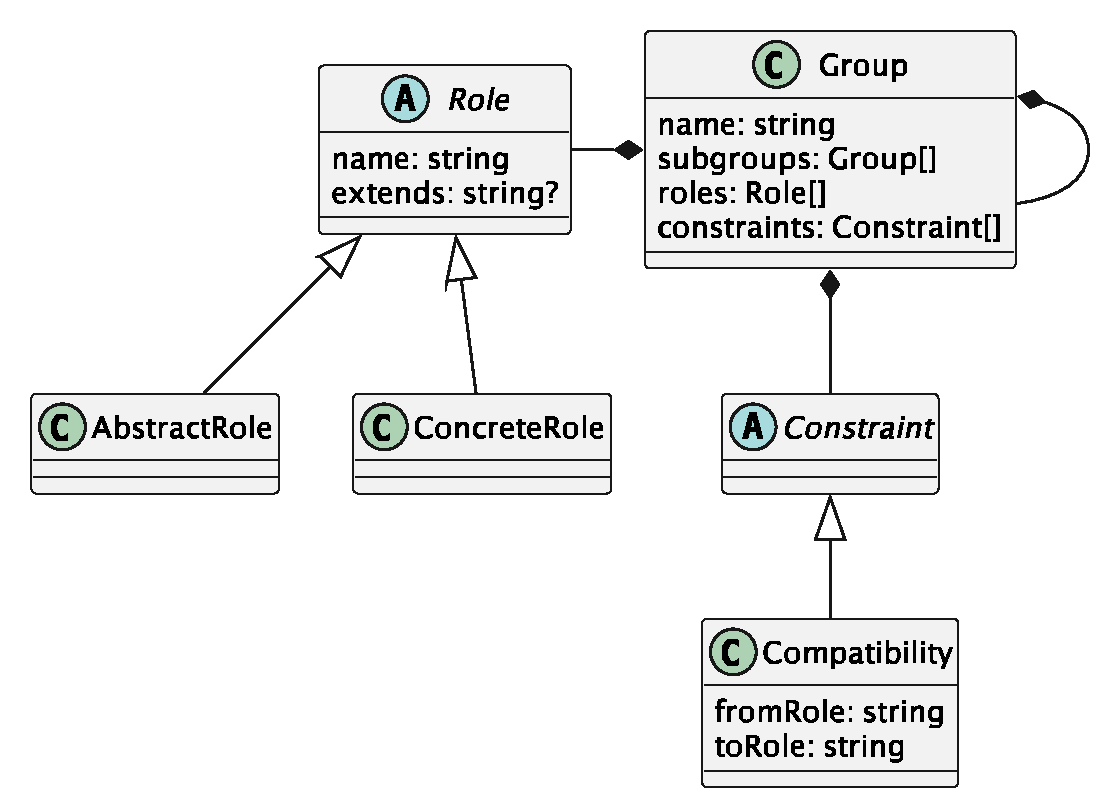
\includegraphics[width=0.9\linewidth]{images/uml/structural-uml.eps}
        \caption{Structural Diagram Core Domain.}
        \label{fig:uml-structural}
    \end{subfigure}
    \begin{subfigure}[h]{0.3\linewidth}
        \centering
        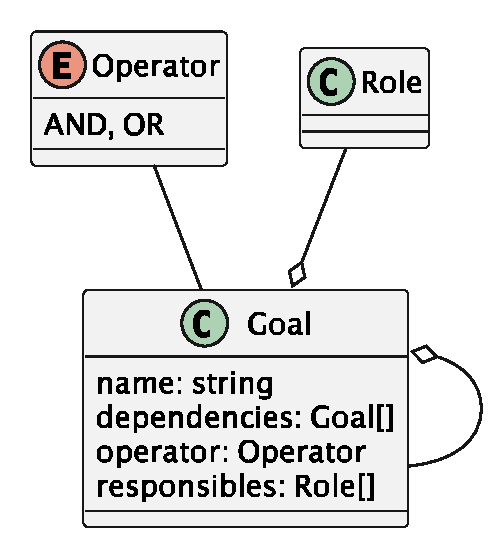
\includegraphics[width=0.9\linewidth]{images/uml/functional-uml.eps}
        \caption{Functional Diagram Core Domain.}
        \label{fig:uml-functional}
    \end{subfigure}
    \caption{UML class diagrams of the core domain.}
    \label{fig:uml-core-domain}
\end{figure}

Specifically, the system keeps track of the components of the diagrams and the relations between them in a list.
The latter is then taken as input by a \texttt{serialize} function that transforms the list into an XML string.
On the other hand, an analogous process is performed when loading an XML specification.
The \texttt{deserialize} function takes the XML string as input and transforms it into a list of components.
In \cref{lst:code-serialization} and \cref{lst:code-deserialization} are shown the functions for the code generation and parsing of the roles inside a group, respectively.

\begin{figure}[H]
    \lstinputlisting[language=Typescript,label={lst:code-serialization},caption={Code generation for the roles inside a group.}]{code/serialization.ts}
\end{figure}

\begin{figure}[H]
    \lstinputlisting[language=Typescript,label={lst:code-deserialization},caption={Parsing of the XML specification of a role inside a group}]{code/deserialization.ts}
\end{figure}

As far as the goal dependencies are concerned, a one-to-one mapping was not possible since the visual language's semantics differs from the one used by \moise{}.
Specifically, the visual language does not allow for the creation of plans and subgoals that are not associated with a specific goal with a plan operator.
In order to overcome this incompatibility, the \textit{depends-on} concept of \moise{} was used.
Although it is usually not directly used in the XML specifications, \textit{depends-on} is a fundamental concept of \moise{} which plans and subgoals are built upon.

Therefore, this concept is used as a mapping between the visual language and the XML syntax.
In particular, when expressing the \textit{and} dependency, a simple \textit{depends-on} tag is created between the two goals.
On the other hand, when expressing the \textit{or} dependency, an intermediate goal is created with a \textit{choice} plan.

For instance, in \cref{lst:goals-and} is shown the XML translation of an \textit{and} dependency between the goals \textit{g1}, \textit{g2} and \textit{g3} of the type:
$$g3 = g1 \wedge g2$$
whereas in \cref{lst:goals-or} is shown the XML translation of an \textit{or} dependency between the goals \textit{g1}, \textit{g2} and \textit{g3} of the type:
$$g3 = g1 \vee g2$$

\begin{figure}
    \lstinputlisting[language=XML,label={lst:goals-and},caption={XML translation of an \textit{and} dependency.}]{code/goals-and.xml}
\end{figure}

\begin{figure}
    \lstinputlisting[language=XML,label={lst:goals-or},caption={XML translation of an \textit{or} dependency.}]{code/goals-or.xml}
\end{figure}

\section{Storage \& Backend}
Organizations can be saved persistently to be later recovered and edited.
This feature is fundamental for the Web IDE since writing a specification is commonly an iterative process that may require the domain expert to edit some parts of an organization either for bug-fixing or to add new features.

\subsection{Storage}

Since the visual programming environment is based on Web technologies, centralized server-side storage was the most natural choice.
Looking at the system architecture in \cref{fig:architecture}, the \textbf{Specifications' Storage} component is responsible for this functionality.

The storage uses a \textit{MongoDB}~\footnote{\url{https://mongodb.com/}} database to store the generated XML specifications.
For the time being, the database does not store the information about the diagrams, such as the position of the components that would make it easier to load the organization in the same state as it was saved.

Moreover, there is no separation between the specifications created by different users, therefore, in a production environment some form of authentication would be necessary.

Finally, a further improvement of the storage component would be to also allow the user to save organization entities, keeping track of which specific configurations of the organization in different scenarios.

\subsection{Backend}
Since, as already mentioned, the Web IDE is based on Web technologies, a backend seemed the most natural choice to make the frontend and the storage communicate.

The backend was implemented using the \textit{Kotlin}~\footnote{\url{https://kotlinlang.org/}} programming language and the \textit{VertX}~\footnote{\url{https://vertx.io/}} library.
The latter is a reactive library that allows the developer to write asynchronous code and build Web servers quickly.
It was chosen because the research group in St.\ Gallen already had some experience with it, therefore, it would be easier to maintain for other developers.
In particular, the projects built by the team use \textit{Java}~\footnote{\url{https://java.com/}} as the programming language, therefore, the choice of \textit{Kotlin} was a fair tradeoff that allowed using a language that is similar to \textit{Java} but with a more modern and concise syntax.

The backend exposes an HTTP API that allows the frontend to communicate with the storage.
The API that is currently implemented is here described:
\begin{itemize}
    \item \texttt{GET /organizations/:name}: returns the XML specification of the organization with the given name.
    \item \texttt{POST /organizations/:name}: saves the XML specification present in the body to the storage.
    \item \texttt{PUT /organizations/:name}: updates the organization with the given name, substituting it with the XML specification present in the body.
\end{itemize}
Since the \texttt{GET} route returns the XML specification, the runtime environment can also use it as a way to retrieve the specification in a resource-oriented fashion.

\section{Running Organization Entities}
In order for users to be able to run the organizations they create, the Web IDE has to be able to communicate with the runtime environment.
Specifically, it needs information about the running agents to assign them to the correct roles and, subsequently, it needs to enforce the organization on said agents.

\subsection{Runtime Environment}
As already mentioned, the runtime environment, which is based on the JaCaMo platform, contains all the running agents and the deployed artifacts.

This component is currently being developed by the research group in St.\ Gallen.
The name of the platform is \textit{Yggdrasil}~\footnote{\url{https://github.com/Interactions-HSG/yggdrasil}}, which comes from the mythological tree of life, and it aims at providing uniform interaction among heterogeneous agents thanks to Hypermedia MAS.
The idea is to model an environment based on the Agents \& Artifacts metamodel through hypermedia and Web technologies, achieving scalability and uniform access to resources.

Yggdrasil exposes a REST-like API that allows users and agents to navigate the environment and the existing workspaces where artifacts and their operations are described with the Thing Description standard since the model perfectly fits the Agents \& Artifacts metamodel.
Moreover, the platform's API also allows the user to run agents and create and deploy artifacts.

The format used by Yggdrasil to describe the resources in the environment is the \textit{Turtle}~\footnote{\url{https://w3.org/TR/turtle/}} format.
The latter is a textual syntax for RDF that allows a knowledge graph to be represented in a compact and natural text form.

\subsection{Running Agents}
Agents in Yggdrasil, just like artifacts, are contained in workspaces.
Therefore, to get the list of agents that are currently running, the Web IDE has to operate on a workspace and retrieve the list of resources that are contained in it.

By performing a \texttt{GET} request to the \texttt{/workspaces} endpoint, specifying the workspace name in the URL, the Web IDE can retrieve a Turtle representation of the workspace; a short example of the response is shown in \cref{lst:turtle-workspace}.
As can be seen, the workspace, which is the subject of all the triples, \textit{directlyContains} \texttt{hypermedia\_body\_1} and \texttt{hypermedia\_body\_2} which represent two agents currently running.

\begin{figure}
    \lstinputlisting[language=Turtle,label={lst:turtle-workspace},caption={Detail of the Turtle representation of a workspace.}]{code/turtle-workspace.ttl}
\end{figure}

Therefore, the Web IDE can parse the Turtle representation and extract the list of agents that are currently running, filtering them from all the other resources that are contained in the workspace.
Since this list is composed of URIs, \texttt{GET} requests to them can be performed to retrieve the Turtle representation of the agents.
The response of the \texttt{GET} request to the agents provide useful information for the user such as the name of the agents that can be used to recognize them and assign them to the correct roles.

\subsection{Artifacts Creation}
Artifacts in Yggdrasil can be created by performing a \texttt{POST} request to the \texttt{workspace/:workspaceName/artifacts} endpoint, specifying all the necessary information in the body of the request.
For instance, the body should contain the type of artifact that is being created, the name of the artifact, and possible initial parameters that the artifact may need.

As far as the organizational artifacts are concerned, the types of artifacts available are the same as the ones described in \textsf{ORA4MAS}, therefore \texttt{OrgBoard}, \texttt{GroupBoard}, \texttt{SchemeBoard}, and \texttt{NormativeBoard}.
Once the \texttt{OrgBoard} artifact is created, the most correct way to generate the other artifacts is through an action exposed by it.
In particular, the \texttt{OrgBoard} artifact exposes the \texttt{createGroup} and \texttt{createScheme} actions that can be used to create the other artifacts.
A \texttt{NormativeBoard}, on the other hand, is automatically generated when a \texttt{SchemeBoard} is linked to a \texttt{GroupBoard}.

Therefore, to correctly instantiate the organizational artifacts and have them refer to the same organization, the Web IDE has to perform a \texttt{POST} request to the \texttt{workspace/:workspaceName/artifacts} endpoint to create the \texttt{OrgBoard} artifact, and then, once the latter is created, perform a \texttt{POST} request to the \texttt{workspace/:workspaceName/artifacts/:orgName/create*} endpoint to create the other artifacts.

\subsection{Organizations' Deployment}
Deploying an organization is a process that includes the creation of the correct organizational artifacts and the adhesion of the agents to the organization, i.e. playing the established roles in the prescribed groups.

\begin{figure}
    \centering
    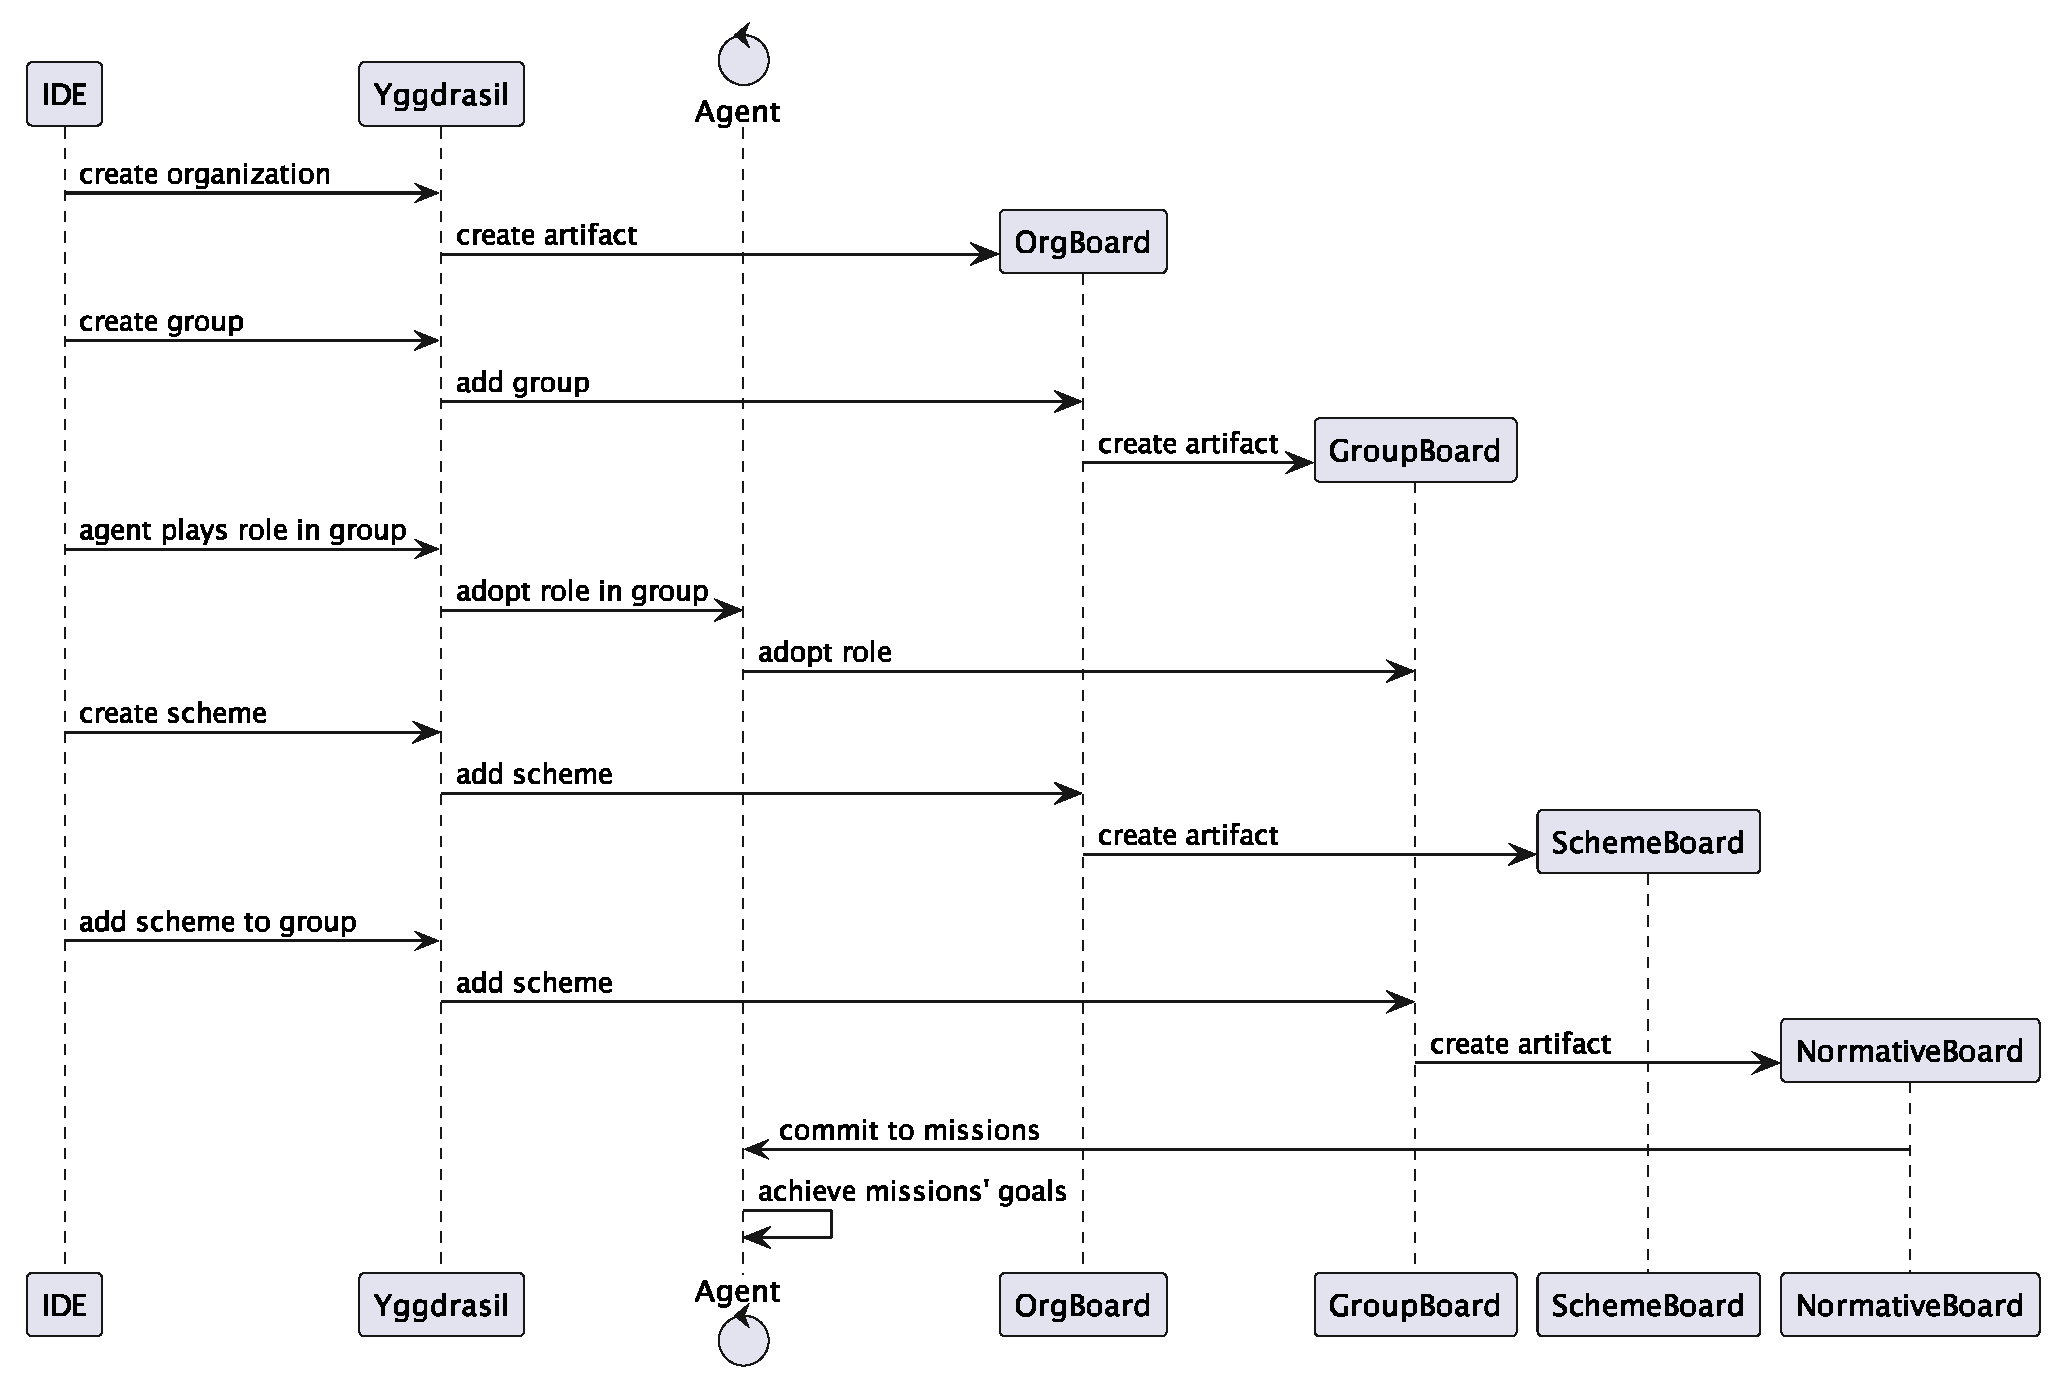
\includegraphics[width=\textwidth]{images/uml/org-creation.eps}
    \caption{Sequence UML diagram of the deployment of an organization. The responses are omitted to improve the readability.}
    \label{fig:org-creation}
\end{figure}

In \cref{fig:org-creation} the typical deployment process of a simple organization is shown.
\begin{enumerate}
    \item The Web IDE first sends a request to Yggdrasil to create the \texttt{OrgBoard} artifact, which is the artifact that represents the organization.
    \item Once the artifact is ready, the Web IDE creates the groups specified in the organization entity.
    For each group, a \texttt{createGroup} request is sent to the \texttt{OrgBoard} artifact, which creates the \texttt{GroupBoard} artifact that represents the group.
    \item The next step involves telling the agents to play the roles specified in the organization entity inside the groups.
    To do so, the Web IDE sends a message to the agents, which know how to send a request to the \texttt{GroupBoard} artifact to play the role.
    \item Subsequently, the Web IDE sends a request to create the scheme of the organization.
    This request is sent to the \texttt{OrgBoard} artifact, which creates the \texttt{SchemeBoard} artifact that represents the scheme.
    \item Finally, the Web IDE sends a request to add the scheme to the groups.
    This request creates a link between the \texttt{SchemeBoard} artifact and the \texttt{GroupBoard} artifacts and a \texttt{NormativeBoard} is automatically generated.
    \item Since the agents are listening to events generated by the \texttt{GroupBoard} artifacts, they will receive a notification telling them to achieve the goals specified in the scheme.
    \item If the agents are obliged to achieve the goals, they will proceed to do so.
    On the other hand, if the agents are permitted to achieve the goals they will do so only if they have an interest in it.
\end{enumerate}

% \section{DevOps}
% In order to 

% In order to make the deployment of the whole system easier, every component has been containerized using \textit{Docker}~\footnote{\url{https://www.docker.com/}}.
% Therefore, a \texttt{Dockerfile} was created for each component, except for the storage component, which only needed the \texttt{mongo} image.

% Moreover, since running every single container with its parameters would be tedious and error-prone, a \textit{Docker Compose}~\footnote{\url{https://docs.docker.com/compose/}} file was created to make the deployment possible with a single command.

% Indeed, the \texttt{docker-compose.yml} file contains all the necessary information to run the whole system,
% such as the images and the build files to use, the ports to expose, the environment variables to set, and the volumes to mount.
% What is more, it takes care of creating a bridge network that allows the containers to communicate with each other.
